\chapter{Аналитический раздел}
\label{cha:analysis}
%
% % В начале раздела  можно напомнить его цель
%
В данном разделе производится анализ процессов распознавания изображения, передачи распознанного изображения, приема изображения и  решения решение его на роботе.
Производится анализ подсистем, входящих в реализуемы программно-аппаратный комплекс, формируются требования к создаваемой системе, выделяются функции её подсистем и описывается взаимодействие между ними.

\section{Общее описание системы}
В рамках данной дипломной работы разрабатывается автономный программно-аппаратный комплекс предоставляющий полный цикл для передачи и распознавания информации, для функционирования которой необходимо спроектировать все подсистемы программного комплекса и способы их взаимодействия.

Для достижения поставленной цели необходимо спроектировать и разработать следующие компоненты системы:
\begin{enumerate}
\item разработать систему распознавания изображения;
\item разработать протокол обмена между роботом и мобильным устройством;
\item разработать систему решения Судоку;
\item разработать систему отрисовки на бумаге полученного решения.
\end{enumerate}


% Обратите внимание, что включается не ../dia/..., а inc/dia/...
% В Makefile есть соответствующее правило для inc/dia/*.pdf, которое
% берет исходные файлы из ../dia в этом случае.


\begin{figure}
  \centering
  \includegraphics[width=\textwidth]{inc/dia/analysis1-1}
  \caption{Схема работы комплекса}
  \label{fig:fig01}
\end{figure}


Так же для удобства и простоты использования комплекса необходимо разработать мобильное приложение и протокол обмена между мобильным устройством и роботом, для того, чтобы стандартизировать сообщения и разрабатывать приложения для любых внешних платформ.

\begin{figure}
  \centering
  \includegraphics[width=\textwidth]{inc/dia/analysis1-2}
  \caption{Компоненты системы}
  \label{fig:fig02}
\end{figure}

\section{Классификация мобильных роботов}
\paragraph{Мобильный робот} - автоматическая машина, в которой имеется движущееся шасси с автоматически управляемыми приводами. Такие роботы могут быть колёсными, шагающими и гусеничными (существуют также ползающие, плавающие и летающие мобильные робототехнические системы).

\paragraph{Микроконтроллер, микрокомпьютеры (англ. Micro Controller Unit, MCU)} — микросхема, предназначенная для управления электронными устройствами. Типичный микроконтроллер сочетает на одном кристалле функции процессора и периферийных устройств, содержит ОЗУ и (или) ПЗУ. 

Поскольку основная масса роботов отличается микроконтроллерами, введем классификацию по этому управляющему элементу.

Существующие робототехнические комплексы:
\begin{itemize}
\item LEGO Mindstorms;
\item fischertechnik.
\end{itemize}

\subsection{LEGO Mindstorms}

\paragraph{LEGO Mindstorms} - конструктор (набор сопрягаемых деталей и электронных блоков) для создания программируемого робота. 

Наборы LEGO Mindstorms комплектуются набором стандартных деталей LEGO (балки, оси, колеса, шестерни) и набором, состоящим из сенсоров, двигателей и программируемого блока. Наборы делятся на базовый и ресурсный.

Все наборы содержат в себе одну и ту же версию интеллектуального блока NXT, отличаются только версии прошивки, но это не принципиально, так как прошивку можно легко обновить. Так что в этом плане все наборы совершенно равноценны. 

В состав наборов могут входить управляющие блоки различных версий. В настоящее время их 3. Также у блоков существуют модификации (обозначается 1.0; 2.0 и т. д.)

Управляющие блоки:
\begin{itemize}
\item RCX - первое поколение управляющих блоков, в данный момент почти не используются из-за устаревшей конструкции модели;
\item NXT - вторая версия коммерческого набора и самое распространенное поколение, 619 деталей в базовом комплекте, год выпуска 2009;
\item EV3 - третье поколение, эволюция модели NXT, более 550 деталей, представлен в сентябре 2013 года.
\end{itemize}
Наборы LEGO Mindstorms располагают огромным количеством сенсоров как компании LEGO, так и сторонних производителей (HiTechnic, Mindsensors и др.). 

\subsection{fischertechnik}

\paragraph{fischertechnik} — пластмассовый развивающий конструктор для детей, подростков и студентов, изобретенный профессором Артуром Фишером в 1964 году. Наборы \textbf{fischertechnik} выпускает немецкая фирма \textbf{fischertechnik GmbH}, которая входит в состав крупного холдинга \textbf{fischertechnik GmbH \& Co.KG}, дочерние фирмы которого выпускают крепёж, крепежный инструмент, детали для автомобилей и различные изделия из пластмассы.

Конструкторы fischertechnik часто используются для демонстрации принципов работы механизмов и машин в средних, специальных и высших учебных заведениях, а также для моделирования производственных процессов и презентационных целей.

Также в комплекты конструкторов входят программируемые контроллеры, двигатели, различные датчики и блоки питания, что позволяет приводить механические конструкции в движение, создавать роботов и программировать их с помощью компьютера.

Имеют только один вид контроллера: \textbf{ROBO TX} - это компактный программируемый контроллер для управления моделями, собранными из конструкторов fischertechnik.

Для разработки управляющих программ для контроллера ROBO TX используется среда программирования \textbf{ROBO Pro}. Готовые программы загружаются в контроллер через интерфейсы USB или Bluetooth.

\subsection{Прочие робототехнические комплексы}

Прочие робототехнические комплексы не представляют никакого интереса для изучения, т.к.  имеют контроллеры специфичной конфигурации, узкое количество сенсоров и наборов, плохо документированные и поддерживаемые узкой группой энтузиастов среды для программирования.

\subsection{Вывод}
Мы будем использовать для написания данного дипломного проекта робототехнический комплекс \textbf{LEGO Mindstorms} по нескольким причинам:
\begin{itemize}
\item большое количество подключаемых модулей, как от самой компании производителя, так и от сторонних компаний;
\item отличная документация на разных языках;
\item самое большое сообщество робототехников, которые поддерживают и развивают данный комплекс;
\item использование альтернативного ПО для программирования роботов.
\end{itemize}

В базовый комплект поставки Mindstorms NXT 2.0 уже включено большинство необходимых деталей для выполнения практически любых задач.

Но так как все описанные роботы располагают малым количеством встроенной FLASH-памяти (256 Кб), а изображение с заданием, которое необходимо будет распознать около 200 Кб, но на FLASH-память нам помимо сжатого изображения придется еще и записывать модули с другими системами, нам придется вывести \textbf{подсистему распознавания} на отдельное мобильное устройство, которое будет обладать достаточной разрешающей способностью для получения изображения нужного качества и обладающего достаточным количеством аппаратных ресурсов, чтобы выполнить возложенные на нее функции.

\section{Подсистема распознавания}
\subsection{Общие представления о системе}

Подсистема распознавания данных должна решать проблему перевода изображений и формирования из него структурированных данных, для последующей передачи другим подсистемам. Таким образом, распознанное изображение должно принять удобный для хранения, использования и передачи, структурированный вид. Результатом работы такой системы должны быть данные, готовые к автоматизированной обработке. 

Общая схема процесса представлена на (рис.~\ref{fig:fig03}).
\begin{figure}[ht]
	\centering
	\includegraphics[width=\textwidth]{inc/dia/analysis1-3}
	\caption{Подсистема сбора данных}
  \label{fig:fig03}
\end{figure}

\subsection{Существующие системы распознавания изображений}

На данный момент существует огромное количество программ, поддерживающих распознавание текста как одну из возможностей. Мы не будем рассматривать такие системы, так как в большинстве своем они избыточны, а наш программно-аппаратный комплекс будет работать в условиях ограниченных аппаратных ресурсов.

\paragraph{OpenCV} (англ. Open Source Computer Vision Library, библиотека компьютерного зрения с открытым исходным кодом) — библиотека алгоритмов компьютерного зрения, обработки изображений и численных алгоритмов общего назначения с открытым кодом. Реализована на C/C++, также разрабатывается для Python, Java, Ruby, Matlab, Lua и других языков. Может свободно использоваться в академических и коммерческих целях — распространяется в условиях лицензии BSD.

\paragraph{JavaANPR}. Реализация – Java. Проект располагается по адресу \url{http://javaanpr.sourceforge.net}. Основное преимущество этой библиотеки в ее кроссплатформенности. Кроме этого, все алгоритмы написаны на Java без использования нативных библиотек, что сильно упрощает использование. Так же эту библиотеку с небольшой доработкой можно использовать на устройствах под управлением OS Android.

Огромный список подобного рода систем показывает, что распознавание информации является популярной и сложной задачей. Для универсального решения данной задачи требуется использовать сложный программно-аппаратный комплекс, требующий огромных вычислительных мощностей(для наших мобильных устройств), что выходит за рамки данной работы и может воплотиться в виде развития рассматриваемой темы. 

\subsection{Возможности системы}

Подсистема распознавания сбора данных должна обеспечивать получение изображение с камеры устройства, распознавание его и сохранение в нужной структуре.  Таким образом приложение, реализующее данную систему, должно работать на мобильном устройстве и должна сохранять изображение в формате, пригодном для дальнейшего решения. 

Для получения чисел из сетки судоку, нам надо определить, а где же наша сетка начинается и кончается. Эта часть является простейшей частью для человеческого мозга, но самой сложной для ПО. Почему? В них слишком много лишних данных. Очень часто газеты и журналы печатают несколько судоку рядом (хм, они явно не рассчитывают на компьютерное распознавание последних). На изображении будет слишком много лишних линий. 

ПО очень сложно определить, какие линии относятся к необходимым нам, а какие являются всего лишь информационным шумом. Где конец нашей сетки и начало следующей.

Каждый алгоритм распознавания имеет три шага:
\begin{itemize}
\item определение необходимых признаков,
\item тренировка,
\item классификация (распознавание в реальном времени).
\end{itemize}

То есть на выходе мы должны иметь упорядоченную структуру в алфавите от 1 до 9.

\subsection{Процесс распознавания}
\begin{figure}[ht]
  \centering
  \includegraphics[width=\textwidth]{inc/dia/analysis1-4}
  \caption{Схема работы подсистемы сбора данных}
  \label{fig:fig04}
\end{figure}
Для получения чисел из сетки судоку, нам надо определить, а где же наша сетка начинается и кончается.  На изображении будет слишком много лишних линий. 

Компьютеру очень сложно определить, какие линии относятся к необходимым нам, а какие являются всего лишь информационным шумом. Где конец нашей сетки и начало следующей.

После того, как мы определили границы, запустим алгоритм преобразования чтобы точно определить линии сетки. До сих пор мы не заботились о перекосах и других дефектах изображения. Только об угле поворота. Этот шаг исправит это. Мы получим точные положения линий сетки. Это поможет определить числа в сетке.

После того, как мы определили, где должны находиться числа, нам необходимо распознать их. Это относительно легко. В алфавите только цифры от 1 до 9.

Скорректировать результаты распознавания.

Данный процесс представлен на (рис.~\ref{fig:fig04}).

\subsection{Требования к подсистеме}
В соответствии с проведенным анализом системы и процессов в ней сформулируем требования к подсистеме.

\subsubsection*{Требования к реализации}
\begin{enumerate}
 \item подсистема распознавания должна выполняться в виде отдельного сервиса;
 \item новые данные должны распознаваться как можно быстрее;
 \item она должна быть гибкой к изменениям угла обзора и поворота;
 \item должен быть разработан удобный интерфейс добавления новых картинок с заданиями;
 \item корректировка результатов OCR (в одной строке, столбце и блоке 3х3 не может находиться одна и та же цифра).
\end{enumerate}

\subsubsection*{Входные данные подсистемы}

\begin{enumerate}
 \item Изображение, полученное с камеры мобильного устройства.
\end{enumerate}

\subsubsection*{Выходные параметры}
\begin{enumerate}
 \item Результат обработки заявки в виде определенной структуры данных;
 \item в случае, если распознавание не прошло полный цикл обработки, данные отправляются для повторного распознавания;
 \item информация о состоянии распознавания.
\end{enumerate}

\section{Подсистема обмена данными}

Главной задачей разрабатываемой системы является предоставление доступа сторонним приложениям доступ к данных, хранящихся на разных компонентах системы. Второй важнейшей задачей является передача данных. Эту проблему призвано решить вторая рассматриваемая подсистема.

В качестве данных в подсистеме обмена выступают распознанные изображения с заданиями, затем нам надо предоставить эти данные подсистеме решения. Такой интерфейс и будет предоставлять текущая подсистема.

Для обменна данными между разными аппаратными модулями единственной и \textbf{беспроводной} спецификацией остается \textbf{Bluetooth}.  

\paragraph{Bluetooth}  —  стандарт коротковолновых технологий, который обеспечивает связь между беспроводными устройствами: мобильными телефонами, КПК, планшетными компьютерами, ноутбуками с поддержкой беспроводной связи, обычными компьютерами и внешними устройствами. Как только связь между двумя устройствами устанавливается, ни одно другое устройство не сможет нарушить эту связь. Устройства не обязательно должны находиться в одном помещении и могут располагаться на расстоянии до 30 метров. Если у вас есть проблемы с использованием Bluetooth, просто щелкните здесь

Так как Bluetooth есть практически в любых совмренных смартфонах, планшетах и мобильных устройствах, то у нас будет доступ к API необходимого устройства и контроллере робота будет свой API, который задействует нужную нам спецификацию.

При создании подсистемы обмена данными наша задача сведется к следующим шагам:
\begin{itemize}
 \item установить сопряжение смартфона и блока управления NXT;
 \item подключиться к блоку NXT;
 \item передать правильную команду;
 \item получить ответ.
\end{itemize}

Наша основная задача сводится к тому, что сформировать структуру сообщений, которыми будут обмениваться устройства для разных задач.
Например, управляющие команды для робота стандартизированы и указаны в спецификации к контроллеру, а вот формат сообщений с заданиями нам надо согласовать, чтобы он был единым между смартфоном и контроллером робота.

\subsection{Cопряжение устройств}
Эту процедуру необходимо проделать один раз на самом первом этапе развертывания системы, в дальнейшем устройства будут уже сопряжены.

Инициализацией bluetooth-соединения принято называть процесс установки связи. Её можно разделить на три этапа:

\begin{itemize}
 \item генерация ключа Kinit;
 \item генерация ключа связи (он носит название link key и обозначается, как Kab);
 \item Аутентификация.
\end{itemize}

Первые два пункта входят в так называемую процедуру сопряжения.

\paragraph{Сопряжение}  — процесс связи двух (или более) устройств с целью создания единой секретной величины Kinit, которую они будут в дальнейшем использовать при общении. В некоторых переводах официальных документов по bluetooth можно также встретить термин «подгонка пары». Перед началом процедуры сопряжения на обеих сторонах необходимо ввести PIN-код.

\subsection{Подключение к блоку NXT}
Подключение к блоку NXT это по большому счету операция сопряжения между устройствами, но нам предоставляется доступ к \textbf{управляющим командам} самого робота.
Формат команд жестко задекларирован  в \cite{Pup09} и \cite{Pup10}. 

\subsection{Обмен данными и командами}

Для обмена информацией и команд между устройствами на контроллере робота предусмотрен определенный формат обмена команд, под который нам нужно будет подстроить устройство с системой распознавания.

\begin{lstlisting}[caption=Формат команд для получения потока данных]
MessageWrite

Byte 0: 0x00 or 0x80
Byte 3: Message size
Byte 4: Message Text
\end{lstlisting}
В данном примере \Code{Byte 0} говорит нам, что это команда прошла успешно, \Code{Byte 3} и \Code{Byte 4} соответственно указывают на размер пересылаемого сообщения и на само сообщение.

\begin{lstlisting}[caption=Формат команды ответа]
Return package:

Byte 0: 0x02
Byte 2: Status Byte
\end{lstlisting}
В ответном сообщении, \Code{Byte 0} указывает нам, что это выходная команда (типа Output) и ее статус \Code{Byte 2}.
Для подсистемы обмена информации нам нужно отправлять заранее заготовленные команды на контроллер робота и сформировать их в отдельный сервис.

\section{Подсистема решения}

\paragraph{Судоку} - популярная головоломка с числами.

Игровое поле представляет собой квадрат размером 9×9, разделённый на меньшие квадраты со стороной в 3 клетки. Таким образом, всё игровое поле состоит из 81 клетки. В них уже в начале игры стоят некоторые числа (от 1 до 9), называемые подсказками. От игрока требуется заполнить свободные клетки цифрами от 1 до 9 так, чтобы в каждой строке, в каждом столбце и в каждом малом квадрате 3×3 каждая цифра встречалась бы только один раз.

Сложность судоку зависит не от количества изначально заполненных клеток, а от методов, которые нужно применять для её решения.

\begin{figure}[ht]
	\centering
	\includegraphics[width=\textwidth]{inc/dia/analysis1-5}
	\caption{Подсистема решения судоку}
  \label{fig:fig05}
\end{figure}

Правильно составленная головоломка имеет только одно решение. Тем не менее, встречаются варианты судоку с несколькими вариантами решения, а также с ветвлениями самого хода решения.

Общая схема процесса представлена на (рис.~\ref{fig:fig05}).

\subsection{Методы решения}
Существует несколько способов решения судоку.

Сложность судоку зависит не от количества изначально заполненных клеток, а от методов, которые нужно применять для её решения. Самые простые решаются дедуктивно: всегда есть хотя бы одна клетка, куда подходит только одно число. 

\subsubsection*{Метод перебора}
Это самый широко используемый программистами способ, который точно даёт решение независимо от уровня сложности. Но перебор может быть очень долгим, это зависит от глубины рекурсии. Вы никогда не узнаете, сколько же итераций вам понадобиться. Во время перебора в клетку ставятся поочерёдно возможные из значений от 1 до 9 и продолжается решение судоку с поставленным числом. Если мы зашли в тупик (получили в одной строке/столбце/блоке одинаковые цифры, то меняем цифру на следующую). На самом деле, может быть больше одного решения.

Во-первых, необходимо подготовить таблицу кандидатов – возможных значений для каждой пустой клетки. Рис.~\ref{fig:fig05}  объясняет, что такое кандидаты. Они окрашены в другой цвет и имеет меньший шрифт. 

\begin{figure}[ht!]
 \centering 
 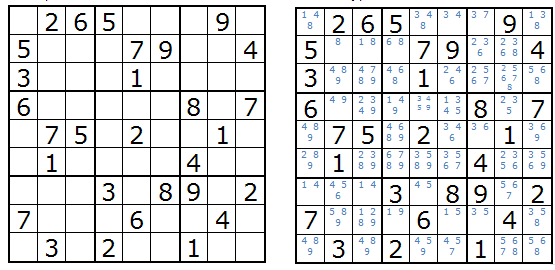
\includegraphics[width=\textwidth]{inc/raster/analysis1-6.png} 
 \caption{Метод перебора} 
 \label{fig:fig06} 
\end{figure}

Метод перебора пробует скомбинировать кандидаты пока не найдёт решения. 

Перебор может быть очень медленным, если решение требует много итераций. 

\subsubsection*{Метод открытых цифр}
Рис.~\ref{fig:fig07}  объясняет этот метод. Если ячейка имеет единственного кандидата, то мы с уверенностью можем сказать, что именно эта цифра должна стоять в этой клетке. После установки значения, следующим шагом будет перестроить список кандидатов. Список кандидатов уменьшается, пока существуют одиночные кандидаты.

Это очевидный и простой метод для машинного решения.

\begin{figure}[ht!]
 \centering 
 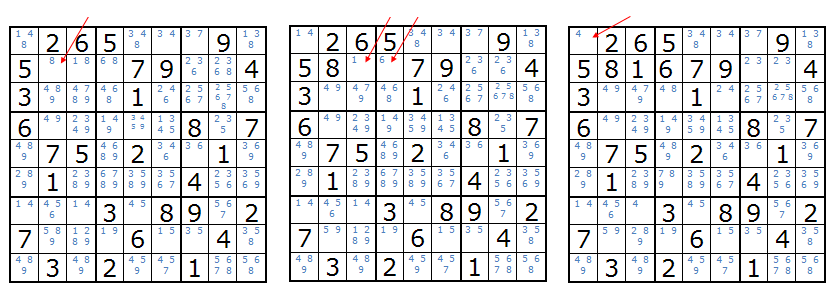
\includegraphics[width=\textwidth]{inc/raster/analysis1-7.png} 
 \caption{Метод открытых цифр} 
 \label{fig:fig07} 
\end{figure}


\subsubsection*{Метод скрытых пар}

Отличным способом раскрыть поле будет поиск скрытых пар. Этот метод позволяет убрать лишних кандидатов из ячейки и дать развитие более интересным стратегиям. Показан на рис.~\ref{fig:fig08}
\begin{figure}[ht!]
 \centering 
 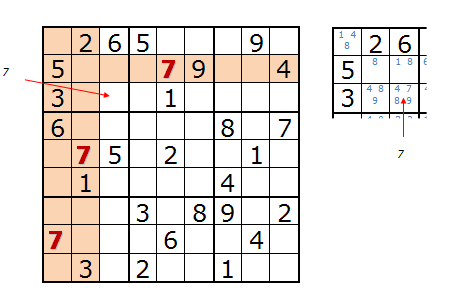
\includegraphics[width=0.5\textwidth]{inc/raster/analysis1-8.png} 
 \caption{Метод скрытых пар} 
 \label{fig:fig08} 
\end{figure}

\subsection{Вывод}
Все описанные методы имеют свои недостатки и преимущества.

Для нас одно из требований для поиска решения - \textbf{скорость обработки}. 

Перебор не слишком быстрый метод. Таким образом, мы будем использовать комбинацию всех трёх методов.

Метод открытых цифр и метод скрытых пар очень быстрые, но могут решать только быстрые пазлы. 

Так как наша подсистема должна решать любые пазлы, нам необходимо скомбинировать решения.

Комбинируя  условия, мы можем утверждать, что в некоторых ячейках  будут только конкретные значения и все другие кандидаты мы убираем.

\section{Подсистема графомоторных навыков}
\subsection{Общие представления о системе}
Одна из главных подсистем в рамках данной дипломной работы это система, которая позволит вывести нам наше решение на лист бумаги. 

\begin{figure}[ht]
	\centering
	\includegraphics[width=\textwidth]{inc/dia/analysis1-9}
	\caption{Общая схема подсистемы графомоторных навыков}
  \label{fig:fig09}
\end{figure}

После получения решения, нашему контроллеру с данной системой предстоит решить несколько задач:
\begin{itemize}
 \item определить ячейку и ее границы;
 \item определить есть ли там цифра из задания или нужно записать;
 \item записать нужную цифру;
 \item определить конец строки/столбца и начать заполнять новый.
\end{itemize}


Общая схема процесса представлена на (рис.~\ref{fig:fig09}).

Для того, чтобы заставить робота двигаться и рисовать плавно, нужно заставить его самому считать скорость движения.

\begin{figure}[ht]
  \centering
  \includegraphics[width=\textwidth]{inc/dia/analysis1-10}
  \caption{Процесс вывода решения на бумагу}
  \label{fig:fig10}
\end{figure}

Процесс вывода решения на бумагу представлен на (рис.~\ref{fig:fig10}).

\subsection{Определение ячеек и их типа}

Функцию зрения на нашем роботе будет осуществлять сенсор цвета.

\paragraph{Сенсор цвета} выполняет три уникальных функции при использовании с блоком NXT.

\begin{enumerate}
  \item может работать как датчик цвета и распознавать шесть цветов;
  \item быть датчиком света, определяющим интенсивность освещения и регистрировать его уровень;
  \item выполнять функции цветной лампы красного, зеленого и синего цветов.
\end{enumerate}

Человек видит черную линию и ее четкую границу. Датчик освещенности работает несколько иначе.

Датчик освещенности видит некое подобие градиента от белого до черного. 

На рис.~\ref{fig:fig11} показана разница в восприятии черной границы для человеческого глаза и робота.

\begin{figure}
  \centering
  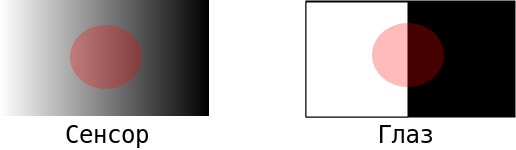
\includegraphics[width=0.65\textwidth]{inc/svg/analysis1-11}
  \caption{Граница для человеческого глаза и сенсора цвета}
  \label{fig:fig11}
\end{figure}

Именно это свойство датчика освещенности – невозможность четко различить границу белого и черного – мы и будем использовать для расчета скорости движения.

Введем понятие \textbf{идеальной точки траектории}.

\paragraph{Идеальная точка} – условная точка примерно посередине белого и черного цветов, следуя которой робот будет регулировать скорость при приближении черной линии.

\subsubsection*{Описание задачи}
\begin{itemize}
\item рассчитать мощность вращения каждого из двигателей с учетом степени отклонения от идеальной точки.	
\end{itemize}


\subsubsection*{Исходные данные}
\begin{itemize}
\item идеальная точка;
\item текущие показания датчика освещенности.	
\end{itemize}

\subsubsection*{Результат}
\begin{itemize}
\item мощность вращения мотора по одной оси;
\item мощность вращения мотора по перпендикулярной оси.	
\end{itemize}



%%% Local Variables:
%%% mode: latex
%%% TeX-master: "rpz"
%%% End:
